\documentclass{article}
%
%   get various packages
%
\usepackage[margin=0.75in]{geometry}                                     % adjust margins
\geometry{letterpaper}                                                  % ... or a4paper or a5paper or ... 
\usepackage{url}                                                        % need this to use URLs in bibtex
\usepackage{setspace}                                                   % need this for \setstrech{...}
\usepackage{scrextend}                                                  % need this for addmargin
\usepackage[export]{adjustbox}                                          % need this to get frame for includegraphics
\usepackage{bigints}                                                    % bigger integral symbol
%
%   tikz et al
%
\usepackage{tikz}
\usetikzlibrary{calc,patterns,angles,quotes,shapes,
                math,decorations,through,intersections,
                lindenmayersystems,backgrounds}    
\usepackage{pgfplots}
\usepackage{pgfplots}	
%
%	math stuff
%
\usepackage{amsmath,amsfonts,amssymb,amsthm}
\usepackage{mathtools}
\usepackage{commath}                                                    % get \norm{x}
\usepackage{fixmath}                                                    % get \mathbold
\usepackage{gensymb}                                                    % get \degree
\usepackage{circuitikz}                                                 % draw circuits
\usepackage{mathrsfs}
\usepackage{hyperref}
\usepackage{url}
\usepackage{subcaption}
\usepackage{authblk}
\usepackage{amsmath}
\usepackage{mathtools}
\usepackage{graphicx}
\usepackage[export]{adjustbox}
\usepackage{hyperref}
\usepackage{alltt}
\usepackage{color}
\usepackage[utf8]{inputenc}
\usepackage[english]{babel}
\usepackage{float}
\usepackage{bigints}
\usepackage{braket}
\usepackage{siunitx}
\usepackage{relsize}
\usepackage{multirow}
%
%	watermarks
%
% \usepackage{draftwatermark}
% \SetWatermarkText{Draft}
% \SetWatermarkScale{5}
% \SetWatermarkLightness {0.9} 
% \SetWatermarkColor[rgb]{0.7,0,0}
%
%
%
%	theorems, definitions, etc
%
\theoremstyle{definition}
\newtheorem{theorem}{Theorem}[section]
\newtheorem{definition}{Definition}[section]
\newtheorem{proposition}{Proposition}[section]
\newtheorem{lemma}{Lemma}[section]
\newtheorem{example}{Example}[section]
\newtheorem{remark}{Remark}[section]
%
\newcommand{\argmax}{\operatornamewithlimits{argmax}}
\newcommand{\argmin}{\operatornamewithlimits{argmin}}
%
%	handy command
%
\newcommand*{\Scale}[2][4]{\scalebox{#1}{$#2$}}%

%
%	title, etc
%
\title{A Few Notes on Simple Harmonic Oscillators}
\author{David Meyer \\ \href{mailto:dmm613@gmail.com}
                            {dmm613@gmail.com}}
\date{Last update: \today}
%
%	be compatible
%
\pgfplotsset{compat=1.17} 
%
%
\begin{document}
\maketitle
%
%
%
\section{Introduction}
This story begins somewhere around 1658 when Robert Hooke
\cite{robert_hooke} began experimenting with springs and
masses. By 1660 Hooke had made two significant steps, namely the
use of a balance controlled by a spiral spring and an improved
escapement called the anchor escapement. In 1660 he discovered an
instance of what we now call Hooke's Law while working on designs
for the balance springs of clocks. However he only announced the
general law of elasticity in his lecture Of Spring given in 1678
\cite{hooke_of_spring}.

\bigskip
\noindent
Interestingly, it was the addition of the balance spring to the
balance wheel around 1658 by Robert Hooke (and Christiaan Huygens
\cite{wiki:huygens}) that greatly increased the accuracy of
portable timepieces, transforming early pocket watches from
expensive novelties to useful timekeepers.


\bigskip
\noindent
These notes are organized (I hope) as follows: Section
\ref{sec:hookes_law} looks at Hooke's Law in some detail.
Section \ref{sec:smo} considers some examples of simple harmonic
oscillators, including Section \ref{subsec:simple_pendulum} which
looks at the simple pendulum, and Section \ref{subsec:lc_circuit}
which considers LC circuits. Section
\ref{sec:quantum_harmonic_oscillators} looks at the Quantum
Harmonic Oscillator. Section \ref{sec:quantum_fields} outlines
how quantum fields fit into all of this. Finally, Section
\ref{sec:conclusions} offers a few observations and conclusions.


\section{Hooke's Law}
\label{sec:hookes_law}
Hooke's law \cite{wiki:hookes_law} is a law of physics that
states that the force needed to extend or compress a spring by
some distance scales linearly with respect to that distance. More
specifically: $F = -kx$, where $k$ is a constant characteristic
of the spring (i.e., its stiffness) and $x$ is the displacement
from the equilibrium point (see Figure
\ref{fig:spring_and_mass_system}).  The law is named after
17th-century British physicist Robert Hooke
\cite{robert_hooke}. Hooke first stated the law in 1676 as a
Latin anagram, and he published the solution of his anagram in
1678 as: ut tensio, sic vis ("as the extension, so the force" or
"the extension is proportional to the force")
\cite{hooke_of_spring}.

\subsection{The Mathematics of Hooke's Law}
\label{subsec:mathematics_of_hookes_law}
\bigskip
\noindent
Hooke's Law describes a form of one-dimensional (scalar) simple
harmonic motion, which as mentioned above occurs when the
restoring force in a system (the force directed toward a stable
equilibrium point) is proportional to the displacement from that
equilibrium. Hooke's Law is most frequently stated as\footnote{In
physics it appears to be convention to use $x$ when $x$ is a scalar 
and $\mathbf{x}$ when it is a vector in force and energy
equations.} $F \propto -x$. That is, the force $F$ is
proportional to the displacement $x$ (hence Hooke's Law describes
simple harmonic motion aka simple harmonic oscillation).  More
frequently this relationship is converted into an equality by the
use of a constant $k$ so that we have


\begin{equation}
F =-kx
\label{eqn:hookes_law}
\end{equation}


\bigskip
\noindent
We also know that Newton's 
Second Law of Motion \cite{wiki:newtons_laws} 
tells us that 

\begin{equation}
F = ma
\label{eqn:newtons_2nd_law}
\end{equation}

\medskip
\noindent
Setting Newton's force (Equation (\ref{eqn:newtons_2nd_law})) 
equal to Hooke's force (Equation (\ref{eqn:hookes_law})) 
gives us

\begin{equation}
ma = -kx
\label{eqn:balancing_force}
\end{equation}

\medskip
\noindent
This implies that

\begin{equation*}
\begin{array}{llll}
ma
&=& -kx
        &\hspace{8em} \mathrel{\#} \text{Equation (\ref{eqn:balancing_force})} \\
[7pt]
&\Rightarrow& a = - \dfrac{k}{m} x
        &\hspace{8em}\mathrel{\#} \text{solve for $a$, noting
                                        that $a$ and $x$ are
                                        functions of time} \\  
[7pt]
&\Rightarrow& \dfrac{d^2 x}{dt^2} = - \dfrac{k}{m} x	
        &\hspace{8em}\mathrel{\#} a
        = \dfrac{d}{dt} \left [ v \right ]
        = \dfrac{d}{dt} \left [ \dfrac{dx}{dt} \right ]
        = \dfrac{d^2 x}{dt^2} \\
\end{array}
\end{equation*}

\bigskip
\noindent
This setup is shown modeling a spring and mass
system\footnote{Where the force is proportional to the distance
$x$ that the spring is stretched from its equilibrium position.}
in Figure \ref{fig:spring_and_mass_system}.


\bigskip
\begin{figure}[H]
\centering
  \resizebox{0.85 \textwidth}{!} {                                                              % resize figure if you want
   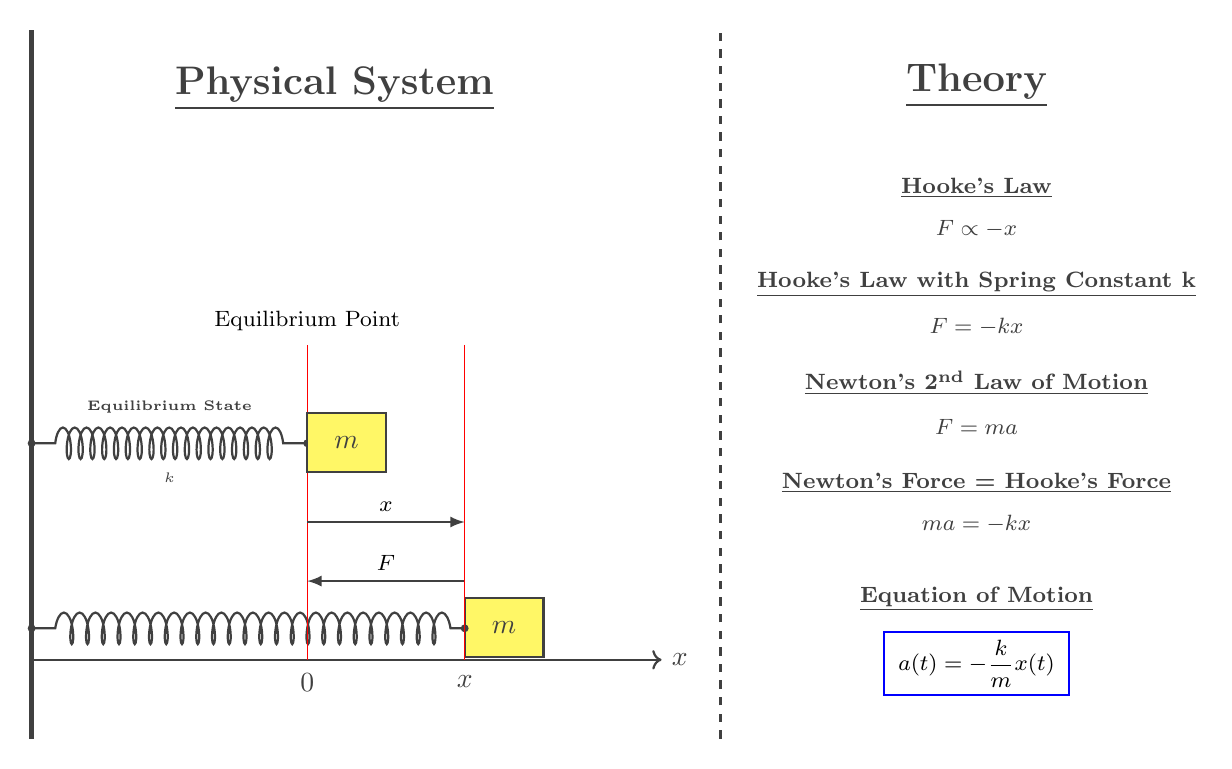
\begin{tikzpicture}[black!75,thick]                                                          % make a picture
        \draw[thick, ->] (0.00,0.00) -- (8.00,0.00) coordinate [label={[right] $x$}];           % draw x axis
        \draw[ultra thick] (0.00,-1.00) -- (0.00,8.00);                                         % this is the support
%
% draw the first spring 
%
        \draw [
              decoration={
                 coil,
                 aspect=0.3, 
                 segment length=2mm, 
                 amplitude=2mm, 
                 pre length=3mm,
                 post length=3mm},
             decorate] (0,0.40) -- (5.75,0.40);
        \fill (0.00,0.40) circle(0.05);                                 						% draw a dot connecting the spring to the vertical support
 %      
 %      draw the first mass
 %
       \node[draw,
	     fill=yellow!60,
	     minimum width=1cm,
	     minimum height=0.75cm,
	     anchor=north,
	     label=center:$m$] at (6,0.80) {};
	     
      \fill (5.5,0.40) circle(0.05);   
      \path (5.5,0.0) node[yshift=-0.75mm, below] {$x$}; 
%
%	make some coordinates
%        
      \coordinate (c1) at (6.00,7.25);
      \coordinate (c2) at (3.50,0.00);
      \coordinate (c3) at (3.50,4.00);            
%
%       draw some text
%  
      \path (c1) node[left] {\Large {\bf \underline{Physical System}}};
      \path (c2) node[yshift=-0.5mm, below] {$0$};
      \draw[thin,red] (c2) -- (c3) coordinate [label={[above, yshift=0.5mm] \text{{\footnotesize \color{black}{{Equilibrium Point}}}}}];   
      \draw[-latex]   (3.50,1.75) -- (5.50,1.75) coordinate [label={[font=\footnotesize,color=black,midway,above] {$x$}}];
      \draw[latex-]   (3.50,1.00) -- (5.50,1.00) coordinate [label={[font=\footnotesize,color=black,midway,above] {$F$}}]; 
      \draw[thin,red] (5.50,4.00) -- (5.50,0.00);
%
% draw the second spring 
%
        \draw [
              decoration={
                 coil,
                 aspect=0.3, 
                 segment length=1.5mm, 
                 amplitude=2mm, 
                 pre length=3mm,
                 post length=3mm},
             decorate]    (0.00,2.75) -- (3.50,2.75);
        \draw [draw=none] (0.00,2.75) -- (3.50,2.75) coordinate [label={[midway,above, yshift=0.25cm] \text{{\tiny {\bf Equilibrium State}}}}];
        \fill (0.00,2.75) circle(0.05);                                         % draw a dot connecting the spring to the y axis
        \fill (3.50,2.75) circle(0.05);                                         % draw a dot connecting the spring to the mass
        \draw [draw=none] (0,2.75) -- (3.5,2.75) coordinate [label={[midway,below,yshift=-0.25cm] {\tiny $k$}}];	% draw k

 %
 % draw the second mass
 %
       \node[draw,
	     fill=yellow!60,
	     minimum width=1cm,
	     minimum height=0.75cm,
	     anchor=north,
	     label=center:$m$] at (4.00,3.15) {};
%	
%	draw information about the graphic to the right ((12.50,Y))
%
%	mostly eyeballed
%
        \draw[dashed,thick] (8.75,-1.00) -- (8.75,8.00);						% draw dashed vertical separator
        \begin{footnotesize}
% 
%	draw header
%
	      \draw [draw=none] (12.00,6.90) -- (12.00,6.90) coordinate [label={[font=\Large, midway] {\bf \underline{Theory}}}]; 
%	
%	draw the rest
%	      
	      \draw [draw=none] (12.00,5.75) -- (12.00,5.75) coordinate [label={[midway] \underline{{\bf Hooke's Law}}}]; 
   	      \draw [draw=none] (12.00,5.25) -- (12.00,5.25) coordinate [label={[midway] {${\displaystyle F \propto -x}$}}];
	      \draw [draw=none] (12.00,4.50) -- (12.00,4.50) coordinate [label={[midway] \underline{{\bf Hooke's Law with Spring Constant $\mathbf {k}$}}}]; 
	      \draw [draw=none] (12.00,4.00) -- (12.00,4.00) coordinate [label={[midway] {${\displaystyle F = -kx}$}}];
	      \draw [draw=none] (12.00,3.25) -- (12.00,3.25) coordinate [label={[midway] \underline{{\bf Newton's ${\mathbf 2^{\text{nd}}}$ Law of Motion}}}]; 
	      \draw [draw=none] (12.00,2.75) -- (12.00,2.75) coordinate [label={[midway] {${\displaystyle F = ma}$}}];	      
	      \draw [draw=none] (12.00,2.00) -- (12.00,2.00) coordinate [label={[midway] \underline{{\bf Newton's Force = Hooke's Force}}}];
	      \draw [draw=none] (12.00,1.50) -- (12.00,1.50) coordinate [label={[midway] {${\displaystyle ma = -kx}$}}];
	      \draw [draw=none] (12.00,0.50) -- (12.00,0.50) coordinate [label={[midway] \underline{{\bf Equation of Motion}}}]; 
	      \draw [draw=none] (12.00,0.00) -- (12.00,0.00) node[draw,rectangle,blue,midway,yshift=-0.05cm] 
                                {${\; \color{black}{a(t) = -\dfrac{k}{m} x(t) \;}}$};			 
        \end{footnotesize}
    \end{tikzpicture}
  }                                                             			% end resizebox
\caption{Spring and Mass System with Spring Constant $k$ and Mass $m$}
\label{fig:spring_and_mass_system}
\end{figure}


\bigskip
\noindent
So now we know that

\begin{equation}
\dfrac{d^2 x}{dt^2} = - \dfrac{k}{m} x
\label{eqn:d2xdt2}
\end{equation}

\bigskip
\noindent
The next question is how do we solve the second order ordinary
differential equation (Equation (\ref{eqn:d2xdt2})) for $x(t)$?
Well, if we imagine the displacement ($x(t)$) plotted on the y
axis against $t$ (plotted on the x axis) we see the familiar
pattern shown in Figure \ref{fig:smh_displacement_function}.
%
%	draw x(t) vs t
%
\bigskip
\begin{figure}[H]
\centering
  \resizebox{0.435 \textwidth}{!} {																	% resize figure if you want
  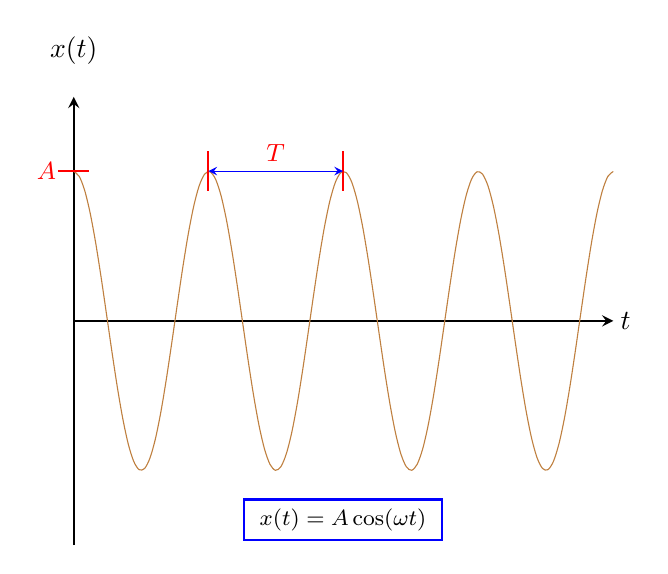
\begin{tikzpicture}
    \def \A {1.0}																					% x(t) = A cos (wt)
    \def \w {1.0}																					% x(t) = A cos (wt)
    \begin{axis}[
      axis line style = thick,
      ticks=none,
      ymin=-1.5,
      ymax=1.5,
      axis x line=middle,
      axis y line=middle,
      xlabel=$t$,
      ylabel={$x(t)$},
      every axis x label/.style={
        at={(ticklabel* cs:1.05)},
        anchor=east,
      },
      every axis y label/.style={
        at={(ticklabel* cs:1.05)},
        anchor=south,
      },
    ]
   \addplot[domain=0:(4*2*pi),samples=100,smooth,brown]{\A*cos(\w*deg(x))};
 \end{axis}
%
%
%
% \fill [red] (0.0,4.75) circle (0.05);															% draw a dot at (0,1) (not really sure how to compute this)
%
  \path (0.0,4.75) node[font=\small,xshift=-1.0mm,left,red] {${A}$};							% label with A
  \draw[thick,red] (-0.20,4.75) -- (0.20,4.75);													% draw a short line
% 
% \fill [red] (1.71,4.75) circle (0.05);														% again, not really sure how to compute these (eyeballed)
% \fill [red]  ({2*1.71},4.75) circle (0.05);
  \draw[thick,red] (1.71,4.50) -- (1.71,5.00); 
  \draw[thick,red] ({2*1.71},4.50) -- ({2*1.71},5.00); 
  \draw[blue,stealth-stealth] (1.71,4.75) -- ({2*1.71},4.75)
                coordinate [label={[font=\small,midway] {${\color{red}{T}}$}}];
  \draw[draw=none] (0.00,0.05) -- ({4*1.71},0.05) 
                coordinate [label={[draw,blue,thick,rectangle,font=\footnotesize,midway]
                {\color{black}{$\; x(t)
                = A \cos (\omega t) \; $}}}];
 \end{tikzpicture}
}
\caption{Simple Harmonic Oscillator Displacement Function}
\label{fig:smh_displacement_function}
\end{figure}

\bigskip
\noindent
Here we can think of the spring being stretched to its maximum
displacement $(A)$ and then let go at time $t = 0$. The mass
($m$) will continue oscillating since in the Hooke's Law setup
the only force acting on the mass is the force due to the spring,
that is, $-kx$. This force is frequently referred to as the
\emph{restoring} force and is shown in Figure
\ref{fig:spring_and_mass_system}.



\bigskip
\noindent
We can check to see if our guess, $x(t) = A \cos (\omega t)$, is
really a solution to Equation (\ref{eqn:d2xdt2}) as follows:

\begin{equation*}
\begin{array}{llll}
\dfrac{d^2 x}{dt^2}
&=& - \dfrac{k}{m} x            &\qquad \qquad \qquad \mathrel{\#} \text{Equation (\ref{eqn:d2xdt2})} \\
[8pt]
&\Rightarrow& \dfrac{d^2}{dt^2}  \Big [A \cos (\omega t) \Big ] = -\dfrac{k}{m} x
				&\qquad \qquad \qquad \mathrel{\#} \text{guess that $x(t) = A \cos (\omega t)$} \\
[8pt]
&\Rightarrow& \dfrac{d}{dt}  \Big [-\omega A \sin (\omega t) \Big ] = -\dfrac{k}{m} x
				&\qquad \qquad \qquad \mathrel{\#} \text{$\dfrac{d}{dt}\cos (u) 
                                = -\sin (u) \dfrac{du}{dt}$ with $u = \omega t$}  \\
[8pt]
&\Rightarrow& -\omega^2 A \cos (\omega t) = -\dfrac{k}{m} x
				&\qquad \qquad \qquad
                                \mathrel{\#} \text{$\dfrac{d}{dt}\sin (u)
                                = \cos (u) \dfrac{du}{dt}$ with $u = \omega t$}  \\
[8pt]
&\Rightarrow& \omega^2 A \cos (\omega t) = \dfrac{k}{m} x
                                &\qquad \qquad \qquad \mathrel{\#} \text{cancel minus} \\
[8pt]
&\Rightarrow& \omega^2 x = \dfrac{k}{m} x
                                &\qquad \qquad \qquad \mathrel{\#} x(t) = A \cos (\omega t) \\
[8pt]
&\Rightarrow& \omega^2  = \dfrac{k}{m}
                                &\qquad \qquad \qquad \mathrel{\#} \text{cancel $x$} \\
[8pt]
&\Rightarrow& \omega  = \sqrt{\dfrac{k}{m}}
                                &\qquad \qquad \qquad \mathrel{\#} \text{take the square root of both sides}
\end{array}
\end{equation*}

\bigskip
\noindent
So $x(t) = A \cos (\omega t)$ is indeed a solution to Equation
(\ref{eqn:d2xdt2}) in the case that

\bigskip
\begin{equation}
\omega  = \sqrt{\dfrac{k}{m}}	
\label{eqn:omega0}
\end{equation}

\bigskip
\noindent
Here $A$ is the maximum displacement (or amplitude) and $\omega$
is the angular frequency (in radians per second). Angular frequency 
is defined to be


\begin{equation}
\omega = \dfrac{2 \pi}{T} = 2 \pi f
\label{eqn:omega1}
\end{equation}

\bigskip
\noindent
where $T$ is the period (time for one cycle in seconds) and $f$
is the frequency in cycles/second \cite{wiki:angular_frequency}.
Note that $f = \dfrac{1}{T}$ so $f$ has units of
$\text{seconds}^{-1}$.

\bigskip
\noindent
Given this information we can write the displacement function
$x(t)$ as in terms of the frequency $f$ as follows:

\begin{equation*}
x(t) = A \cos (2 \pi f t)
\end{equation*}

\bigskip
\noindent
We can also put Equations (\ref{eqn:omega0}) and (\ref{eqn:omega1}) 
together to find that

\begin{equation*}
f = \dfrac{1}{2 \pi} \sqrt{\dfrac{k}{m}}
\end{equation*}

\noindent
and

\begin{equation*}
T = 2 \pi \sqrt{\dfrac{m}{k}}
\end{equation*}


\section{Total Energy of a Simple Harmonic Oscillator}
We know that the total energy of an oscillator  
such as the spring and mass system we looked 
at above is

\vspace{-0.15cm}
\begin{equation*}
E_{\text{total}} = \text{KE} + \text{PE}
\end{equation*}

\medskip
\noindent
All good, but what is the kinetic energy (KE) and potential
energy (PE) of such as system? Well, we know that 
$\text{KE} = \frac{1}{2} mv^{2}$ \cite{kinetic_energy}, but 
what about the potential energy of the system?

\subsection{Potential Energy of a Simple Harmonic Oscillator}
Potential energy is the energy a system has due to position,
shape, or configuration. It is stored energy that is completely
recoverable.

\medskip
\begin{definition} {\bf Conservative Force:} A conservative force 
is one for which work done by or against the force depends only 
on the starting and ending points of a motion and not on the path 
taken \cite{wiki:potential_energy}.
\end{definition}

\medskip
\noindent
Now we can define the potential energy (PE) for any conservative
force.  The work done against a conservative force to reach a
final configuration depends on the configuration, not the path
followed, and is the potential energy added. So in the case of a
simple harmonic oscillator the work $W$ done by a force $F$ is
equal to $\int_{x} F(x) \; dx$. That is, $W$ equals the area under
$F$ \cite{wiki:conservative_force}. Since work (and therefore
potential energy) is a scalar quantity
\cite{elastic_potential_energy} we are only interested in the
magnitude of $F$, $kx$, at each point $x$ (the sign is the
direction of the $F$ vector in the one dimensional case). So if
we set $F_{1} = kx$ we get the curve shown in Figure
\ref{fig:PE}, where we can see that the area under the curve is
$\frac{1}{2} kx^2$. Thus the work done or potential energy stored
is $\frac{1}{2} kx^2$.
%
%	draw "Potential Energy of a Spring and Mass System"
%	
\begin{figure}[H]
\centering
  \resizebox{0.395 \textwidth}{!} {                              % resize figure if you want
  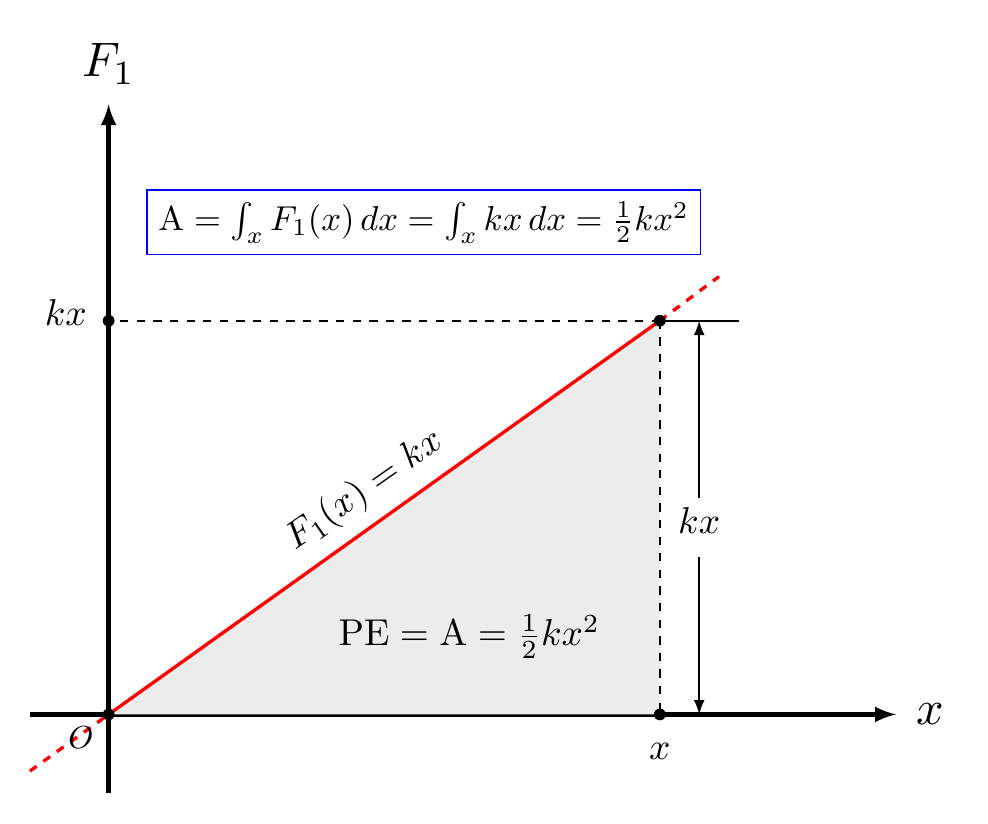
\begin{tikzpicture}
%
%	Set up coordinates
%
       \coordinate (O)                  at (0,0);               % origin O
       \coordinate (Ominus)				at (-1,-.72);			% (5/7)*-1 ≈ -.7142857
       \coordinate (Xstart)             at (-1,0);              % x-axis 
       \coordinate (Xend)               at (10,0);              % x-axis
       \coordinate (Ystart)             at (0,-1);              % y-axis
       \coordinate (Yend)               at (0,7.75);            % y-axis
       \coordinate (EP)                 at (7,5);               % endpoint of the F vs. x line segment of interest
       \coordinate (EPO)                at (8,5);               % endpoint of extension for kx vertical line
       \coordinate (EPL)                at (7.75,5.56);			% endpoint of the F vs. x line: (5/7) * 7.75 ≈ 5.53571429
       \coordinate (TopHalf1)           at (7.5,2.75);          % top half of kx line
       \coordinate (TopHalf2)           at (7.5,5);             % top half of kx line
       \coordinate (BottomHalf1)        at (7.5,2);             % bottom half of kx line
       \coordinate (BottomHalf2)        at (7.5,0);             % bottom halft of kx line
       \coordinate (X)                  at (7,0);               % x coordinate of kx line
       \coordinate (Y)					at (0,5);				% draw a dot on the y axis
       \coordinate (A)					at (4.0,6.25);			% A = ... rectangle
%
%	Draw the axes, shading the lower triangle
%
       \draw[ultra thick,-latex](Xstart) -- (Xend) node[right,scale=1.75] {$x$};		% x axis
       \draw[ultra thick,-latex](Ystart) -- (Yend) node[above,scale=1.75] {$F_{1}$};	% y axis
       \draw [draw=none,fill=gray!15] (O) -- (EP) -- (X) -- cycle;
%
%	Draw the area and the force function
%
       \draw [draw=none] (O) -- (X) node[midway,above,scale=1.35,yshift=0.40cm,xshift=0.80cm] 
       				{${\text{PE} = \text{A} = \frac{1}{2}kx^2}$};
%
%	Label the line segment of interest (F_{m} = kx)
%
       \draw[very thick,red](O) -- (EP) node [left,above,midway,scale=1.35,rotate=35]	
       				{${\color{black}{F_{1}(x) = kx}}$};
%
%	Draw the dashed segments of the line
%
	   \draw[very thick,dashed,red](EP) -- (EPL) node [scale=1.35] {};
	   \draw[very thick,dashed,red](Ominus) -- (O) node [scale=1.35] {};

%
%	Draw dots at the endpoints of the line segment of interest
%
	   \fill [black] (O)  circle (0.075);
       \fill [black] (EP) circle (0.075);
%
%	Draw dashed line from the endpoint of the line segment (EP) down 
%	to the x axis (O)
%       
       \draw[thick,dashed](EP) -- (X) coordinate [];
       \fill [black] (X)  circle (0.075) node [below,yshift=-0.20cm,scale=1.35] {$x$};
%
%	Draw the top horizontal line for the kx arrow
%
       \draw [thick] (EP) -- (EPO) [];
%
%	Label the origin
%
       \node [xshift=-0.35cm,yshift=-0.30cm,scale=1.15] at (0,0) {$O$};
%
%	Surely there is a better way to do this but this is what I came up with
%
       \draw [latex-, thick] (TopHalf2) -- (TopHalf1) node [below,yshift=0.05cm,scale=1.35] {$kx$};
       \draw [-latex, thick] (BottomHalf1) -- (BottomHalf2) [];
%
%	Show kx on the F axis
%
       \draw [thick,dashed] (EP) -- (Y) node [left,xshift=-0.10cm,yshift=0.10cm,scale=1.35] {$kx$};
       \fill [black] (Y) circle (0.075);
%
%	Draw the rectangle with A = ...
%
	   \node [draw,rectangle,blue,scale=1.25] at (A) 
	   		{$\color{black}{\text{A} = 
	   		  \int_{x} F_{1}(x) \, dx =
			  \int_{x} kx \, dx = 
			  \frac{1}{2}kx^{2}}$
			  };   
%
%	done
%       
   \end{tikzpicture}
  }                                                             % end \resizebox
 \caption{Potential Energy of a Simple Harmonic Oscillator}
 \label{fig:PE}
\end{figure}

\bigskip
\noindent
So now we know that $E_{\text{total}} = E(x,v) = \frac{1}{2}mv^2 + 
\frac{1}{2}kx^2$. This implies that

\begin{equation*}
\begin{array}{llll}
E(x,v)
&=& \dfrac{1}{2}mv^2 + \dfrac{1}{2}kx^2 									
						&\hspace{4em} \mathrel{\#} E(x,v) = \text{KE} + \text{PE} \\
[12pt]
&=& \dfrac{1}{2} m \left (\dfrac{dx}{dt} \right )^2 + \dfrac{1}{2}kx^2 		
						&\hspace{4em} \mathrel{\#} v = \dfrac{dx}{dt} \\
[12pt]
&=& \dfrac{1}{2} m \left (\dfrac{d}{dt} \Big [A \cos (\omega t) \Big ] \right )^2 + \dfrac{1}{2}kx^2 
						&\hspace{4em} \mathrel{\#} x(t) = A \cos (\omega t) \\
[12pt]
&=& \dfrac{1}{2} m \left (- \omega A \sin (\omega t) \right )^2 + \dfrac{1}{2}kx^2 
						&\hspace{4em} \mathrel{\#} \text{$\dfrac{d}{dt}\cos (u)
                                                = -\sin (u) \dfrac{du}{dt}$ with $u = \omega t$}  \\
[12pt]
&=& \dfrac{1}{2} m \omega^2 A^2 \sin^2 (\omega t) + \dfrac{1}{2}kx^2 
						&\hspace{4em} \mathrel{\#} \left (- \omega A \sin (\omega t) \right )^2 = 
						                           \omega^2 A^2 \sin^2 (\omega t) \\
[12pt]
&=& \dfrac{1}{2} m \omega^2 A^2 \sin^2 (\omega t) + \dfrac{1}{2}k\left (A \cos (\omega t) \right )^2 
						&\hspace{4em} \mathrel{\#} x(t) = A \cos (\omega t)\\
[12pt]
&=& \dfrac{1}{2} m \omega^2 A^2 \sin^2 (\omega t) + \dfrac{1}{2}k A^2 \cos^2 (\omega t) 
						&\hspace{4em} \mathrel{\#} \left ( A \cos (\omega t) \right )^2 = A^2 \cos^2 (\omega t) \\
[12pt]
&=& \dfrac{1}{2} m \omega^2 A^2 \sin^2 (\omega t) + \dfrac{1}{2} m \omega^2 A^2 \cos^2 (\omega t) 
						&\hspace{4em} \mathrel{\#} \omega = \sqrt{\dfrac{k}{m}} \Rightarrow k = m 
						                           \omega^2 \text{ (Equation (\ref{eqn:omega0}))} \\
[12pt]
&=& \dfrac{1}{2} m \omega^2 A^2 \left (\sin^2 (\omega t) + \cos^2 (\omega t) \right )
						&\hspace{4em} \mathrel{\#} \text{factor out $\dfrac{1}{2} m 
						                           \omega^2 A^2$} \\
[12pt]
&=& \dfrac{1}{2} m \omega^2 A^2
						&\hspace{4em} \mathrel{\#} \sin^2 (\omega t) + \cos^2 (\omega t) = 1 \\
[12pt]
&=& \dfrac{1}{2} m (2 \pi f)^2 A^2 
						&\hspace{4em} \mathrel{\#} \omega = 2 \pi f \\
[12pt]
&=& \dfrac{1}{2} 4 \pi^2 f^2 A^2 m
						&\hspace{4em} \mathrel{\#} \text{expand $\left (2 \pi f \right)^2$ 
						                           and rearrange} \\
[12pt]
&=& 2 \pi^2 f^2 A^2 m
						&\hspace{4em} \mathrel{\#} E_{\text{total}} = 2 \pi^2 f^2 A^2 m\\
[12pt]
&\Rightarrow& E(x,v) \propto f^2 A^2 
						&\hspace{4em} \mathrel{\#} \text{$E(x,v)$ is proportional to $f^2 A^2$}\\

\end{array}
\end{equation*}

\bigskip
\noindent
So we see that the oscillator has $E(x,v) = 2
\pi^2 f^2 A^2 m$, or said another way $E(x,v)\propto
f^2 A^2$. This result will become useful when we consider the
quantum harmonic oscillator.

\bigskip
\noindent
The next section drills down a bit on conservation of energy
in the one-dimensional case.


\subsection{Conservation of Energy: One Particle in One Dimension}
\label{subsec:conservation_of_energy}
The first thing to note here is that since we are in one-dimensional
space (motion is in $\mathbb{R}^{1}$), quantities such as displacement,
velocity, and acceleration, force, and energy are scalars. It seems to 
be convention to use, for example, $F = ma$ rather than 
$\mathbf{F} = m \mathbf{a}$, when working in $\mathbb{R}^{1}$.

\bigskip
\noindent
Next, we will need the following definition:

\medskip
\begin{definition}
{\bf Trajectory:} A solution x(t) to the equation $F(x(t)) = m \ddot{x}(t)$,
Newton’s Second Law, is called a trajectory.
\end{definition}

\medskip
\noindent
Now, consider the case of a general force function $F(x)$. Here we define 
the kinetic energy of a particle to be $\frac{1}{2}mv^{2}$. We also 
define the potential energy of a particle, $V(x)$, to be 


\begin{equation}
V(x) = - \int F(x) \, dx
\label{eqn:V(x)}
\end{equation}

\noindent
so that 

\begin{equation}
\dfrac{d}{dx}V(x) = -F(x)
\label{eqn:F}
\end{equation}

\bigskip
\noindent
Then the total energy of a particle as a function of displacement and 
velocity, $E(x,v)$, is defined to be 

\begin{equation}
E(x,v) = \dfrac{1}{2}mv^{2} + V(x)
\label{eqn:E(x,v)}
\end{equation}

\medskip
\noindent
One of the main reasons this energy function is important is that it is 
\emph{conserved}, meaning that its value along any trajectory is constant.
Switching notation ($x = x(t)$ and $v = \dot{x}(t)$) and saying this in 
a slightly different way: An energy function is \emph{conserved} if, for 
each trajectory $x(t)$ conforming to Newton’s Second Law, a particle's 
total energy $E(x(t),\dot{x}(t))$ is independent of $t$. The conditions
under which the total energy of a particle is conserved is the topic of 
Theorem \ref{theorem:conservation_of_energy_in_R1}.



\medskip
\begin{theorem}
\label{theorem:conservation_of_energy_in_R1}
Suppose a particle's trajectory conforms to Newton’s Second Law 
in the form $F(x(t)) = m\ddot{x}(t)$ and let $V$ and $E$ be as 
in Equations (\ref{eqn:V(x)}) and (\ref{eqn:E(x,v)}). In this 
case the total energy of the particle is conserved.

\bigskip
\noindent
{\bf Proof.} To show that the total energy of the particle is
conserved we want to show that a particle's total energy does 
not change with time, that is, we want to show that 
$\dfrac{d}{dt}E(x(t),\dot{x}(t)) = 0$. As we will see, computing 
this derivative requires a bit of machinery from the chain and 
power rules \cite{wiki:chain_rule,wiki:power_rule}:
%
%
%
\bigskip
%
%
%
\begin{equation*}
\begin{array}{llll}
\dfrac{d}{dt} E(x(t),\dot{x}(t))
&=& \dfrac{d}{dt} \bigg [\dfrac{1}{2}m{(\dot{x}(t))}^{2} + V(x(t)) \bigg ]	
		&\hspace{0em} \mathrel{\#} \text{definition of $E(x(t),\dot{x}(t))$ 
		                                 (Equation (\ref{eqn:E(x,v)}))} \\	
[15pt]
&=& \dfrac{d}{dt} \bigg [ \dfrac{1}{2}m{(\dot{x}(t))}^{2} \bigg ] + \dfrac{d}{dt} V(x(t))
		&\hspace{0em} \mathrel{\#} \text{since derivative is a linear 
		                                 operator \cite{wiki:linearity_of_differentiation}} \\
[15pt]
&=& m\dot{x}(t)\ddot{x}(t) + \dfrac{d}{dt} V(x(t))
		&\hspace{0em} \mathrel{\#} \text{by the power \& chain rules: $\dfrac{d}{dt} 
										\left [ \dfrac{1}{2}m{(\dot{x}(t))}^{2} \right ] = 
										 m\dot{x}(t)\ddot{x}(t)$}\\
[15pt]
&=& m\dot{x}(t)\ddot{x}(t) + \left [ \dfrac{d}{dx} V(x(t)) \right ] \dot{x}(t)
		&\hspace{0em} \mathrel{\#} \text{$\underbrace{\dfrac{dV}{dt} = 
									     \dfrac{dV}{dx} \dfrac{dx}{dt}}_{\text{chain rule}} =
										 \dfrac{dV}{dx}\dot{x} \, \Rightarrow
										 \dfrac{d}{dt} V (x(t)) = 
										 \left [ \dfrac{d}{dx} V(x(t)) \right ] \dot{x}(t)$} \\
[15pt]
&=& \dot{x}(t) \cdot \left [m \ddot{x}(t) + \dfrac{d}{dx}V(x(t)) \right ]
		&\hspace{0em} \mathrel{\#} \text{factor out $\dot{x}(t)$} \\
[15pt]
&=& \dot{x}(t) \cdot \Big [m \ddot{x}(t) - F(x(t)) \Big ]
		&\hspace{0em} \mathrel{\#} \text{since $\dfrac{d}{dx}V(x(t)) = - F(x(t))$ 
		                                 (Equation (\ref{eqn:F}))} \\
[15pt]
&=& \dot{x}(t) \cdot 0
		&\hspace{0em} \mathrel{\#} \text{by Newton's $2^{\text{nd}}$ law: 
		                                 $F = m\ddot{x} \Rightarrow m\ddot{x} - F = 0$} \\
[15pt]
&=& 0
		&\hspace{0em} \mathrel{\#} \dfrac{d}{dt} E(x(t),\dot{x}(t)) = 0 
\end{array}
\end{equation*}

\bigskip
\noindent
So we see that $\dfrac{d}{dt} E(x(t),\dot{x}(t)) = 0$ along any 
trajectory, which implies that $E(x(t), \dot{x}(t))$ is independent 
of $t$. Hence the total energy of the particle is conserved. 
$\blacksquare$
\end{theorem}

% \medskip
\noindent
Energy is sometimes called a \emph{conserved quantity} (or 
\emph{constant of motion}), since a particle neither gains 
nor loses energy as it moves according to Newton’s Second 
Law. 

\section{Other Simple Harmonic Oscillators}
\label{sec:smo}

\subsection{The Simple Pendulum}
\label{subsec:simple_pendulum}
A pendulum is a weight (that is, a mass $m$ in a gravitational
field) suspended from a pivot so that it can swing freely
\cite{wiki:pendulum}.  When a pendulum is displaced sideways from
its resting, equilibrium position, it is subject to a restoring
force due to gravity that will accelerate it back toward the
equilibrium position. When released, the restoring force acting
on the pendulum's mass causes it to oscillate about the
equilibrium position, swinging back and forth. The time for one
complete cycle, a left swing and a right swing, is called the
period ($T$). The period depends on the length of the pendulum
and also to a slight degree on the amplitude ($A$), the width of
the pendulum's swing. The free body diagram
\cite{wiki:free_body_diagram} for the simple pendulum is shown in
Figure \ref{fig:simple_pendulum}.


\bigskip
\noindent
From the first scientific investigations of the pendulum around
1602 by Galileo Galilei, the regular motion of pendulums has been used
for timekeeping. The pendulum clock invented by Christiaan Huygens in 
1658 became the world's standard for timekeeping \cite{wiki:huygens} 
and was used in homes and offices for 270 years until it was supplanted  
by the quartz clock in the 1930s \cite{quartz_crystal_clock}. 
Pendulums are also used in scientific instruments such 
as accelerometers and seismometers. Historically they were used as 
gravimeters to measure the acceleration of gravity in geo-physical 
surveys, and even as a standard of length. The word "pendulum" is 
new Latin, from the Latin \emph{pendulus} meaning 'hanging'
\cite{american_heritage_dictionary}.


\medskip
\bigskip
\begin{figure}[H]
  \centering
  \resizebox{0.50 \textwidth}{!} {																	% resize figure if you want
    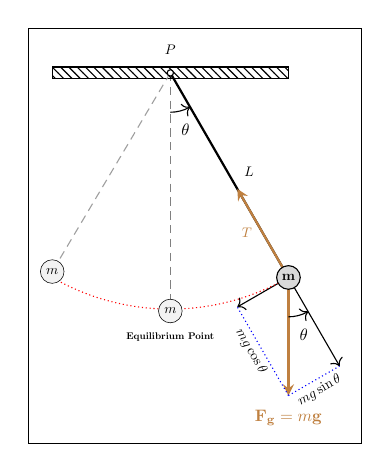
\begin{tikzpicture} [framed] 																	% put a frame on the tikzpicture 
      \pgfmathsetmacro{\Gvec}{1.5}																	% save length of g-vector and theta to macros
      \pgfmathsetmacro{\myAngle}{30}
      \pgfmathsetmacro{\Gcos}{\Gvec*cos(\myAngle)}													% calculate lengths of vector components
      \pgfmathsetmacro{\Gsin}{\Gvec*sin(\myAngle)}
%
%	make some coordinates
%
      \coordinate (P) at (0,0);                                               						% pivot point P is at the origin
%
%	pendulum support, pivot
%
      \draw[thin, densely dashed, gray] (0,0) -- ++(0,-3.0) node (EP) [black, below] {};			% EP is the Equilibrium Point (this connects to bob1)
	  \draw[pattern=north west lines, pattern color=black] (-1.5,-0.075) rectangle (1.5,0.075);		% draw support
	  \path (0.0, 0.25) node[above,yshift=-0.75mm,scale=0.50] {$P$};								% label pivot point P
%
%	draw the pivot below (at end) so that nothing is on top of it
%
%	\filldraw [thin, fill=white,draw] (o) circle[radius=0.050];  % pivot point P = o
%
      \draw[thick] (P) -- ++(270+\myAngle:3) coordinate (bob);
      \path (1.00,-1.25) node[scale=0.50] {$L$}; 
      \draw [thick,brown,-stealth] (bob) -- ($(bob)!\Gcos cm!(P)$) 
        node[left,midway,xshift=-0.75mm,scale=0.50] {$T$};
%
%	draw the angle
%
     \pic [draw, ->, "${\Scale[0.60]{\theta}}$", angle eccentricity=1.5] {angle = EP--P--bob};
%
%	draw the rest of the pendulum (except draw the bob last)
%
     \draw [->] (bob) -- ($(bob)!-\Gcos cm!(P)$)        coordinate (gcos); 
     \draw [->] (bob) -- ($(bob)! \Gsin cm!90:(P)$)     coordinate (gsin);
     \draw [thick,brown,-stealth] (bob) -- ++(0,-\Gvec) coordinate (g)
       node[below,brown,yshift=-1.0mm,scale=0.60] {${\bf F_{g}} = m {\bf g}$};
     \pic [draw, ->, "{$\Scale[0.60] {\theta}$}", angle eccentricity=1.5] {angle = g--bob--gcos};
     \draw [densely dotted, thin, blue] (g) -- (gsin) 
       node[midway,xshift=-0.15cm,rotate=-60,scale=0.50] {$\color{black}{mg \cos \theta}$};
     \draw [densely dotted, thin, blue] (g) -- (gcos) 
       node[midway,below,rotate=30,scale=0.50] {$\color{black}{mg \sin \theta}$};  
%
%	draw bob at origin and on the other side
%
     \draw[red, densely dotted] (bob) arc(-60:-120:3);								% draw arc   
     \coordinate (bob1) at ($(EP) + (0,0.10)$);										% draw bob1 
     \filldraw [very thin, fill=black!5, draw=black] (bob1) circle[radius=0.150];
     \path (bob1) node[scale=0.50] {$m$};
     \path (bob1) node[scale=0.35,below,yshift=-0.65cm] {\bf Equilibrium Point};
%
%	coordinates for bob2 plus line from the pivot to bob2
%
     \coordinate (bob2) at ($(bob) + (-3,{0.150/2})$);
     \draw [thin, densely dashed, gray!75] (P) -- (bob2);
%
%	make sure bob and bob2 are on top, so draw last
%
     \filldraw [thin, fill=white,draw] (P) circle[radius=0.04];							% pivot point p
     \filldraw [fill=black!15,draw=black] (bob) circle[radius=0.150];						% draw bob
     \path (bob) node[scale=0.50] {${\bf m}$};
     
     \filldraw [very thin, fill=black!5,draw=black] (bob2) circle[radius=0.150];                                % draw bob2
     \path (bob2) node[scale=0.50] {$m$};
     
   \end{tikzpicture}
  }                                                                                                             % end \resizebox
 \caption{Free Body Diagram for a Simple Pendulum}
 \label{fig:simple_pendulum}
\end{figure}

\bigskip
\noindent
The simple pendulum setup has a point mass $m$ (the bob) 
on a string (or rod) of length $L$. Here the mass of the string 
is assumed to be negligible as compared  to the mass of the bob. 
The pendulum pivots around a frictionless point $P$ on the support.  
The only forces acting on the bob are the force of gravity 
(i.e., the weight of the bob) and tension from the string (T). 
The forces on the bob result in a net force of $- mg \sin \theta$ 
toward the equilibrium point. This force is called a 
\emph{restoring force} since it points in the direction of the
equilibrium  point. The simple pendulum 
setup is shown in Figure \ref{fig:simple_pendulum}.

\subsubsection{Applying Newton's Laws to the Simple Pendulum}
The pendulum is governed by Newton’s laws applied to 
rotational motion, namely

\begin{equation}
\tau = I \alpha
\label{eqn:tau}
\end{equation}

\bigskip
\noindent
where $\tau$ is the torque, $I$ is the moment of 
inertia, and $\alpha$ is the angular acceleration 
\cite{nave_simple_harmonic_motion}.

\bigskip
\noindent
Torque is interesting. It is a measure of rotational force, that
is, it is a measure of twist. The moment of inertia of an object,
also known as its rotational inertia, is a measure of how
difficult it is to change the rotation of that object. It is an
analogue of mass: mass is to force as rotational inertia is to
torque. Angular acceleration is simply the change in velocity of
the angle $\theta$ of the pendulum and is typically
denoted\footnote{Here again $\theta$ and $\theta(t)$ are used
interchangeably.} by either $\ddot{\theta}(t)$ or
$\frac{d^2 \theta}{dt^2}$. 

\bigskip
\noindent
A torque on a lever can be expressed as $\boldsymbol{\tau} = {\bf
F} \times {\bf r}$, a force {\bf F} multiplied by a distance from
the pivot {\bf r}. In this case (Figure \ref{fig:simple_pendulum}),
${\bf r} = L$ and ${\bf F} = m {\bf g} \sin \theta$, the force due 
to gravity that is perpendicular to the string. This force can be 
found by splitting the total gravitational force into its parallel 
and perpendicular parts through vector algebra (BTW, this is one 
of the reasons to like Lagrangian mechanics over Newtonian 
mechanics; Lagrangian mechanics uses (mostly) scalars whereas 
Newtonian mechanics uses vectors). This operation seems to be 
common and physics. In the case shown in Figure \ref{fig:simple_pendulum} 
we find that ${\bf F} = m {\bf g} \sin \theta$, the perpendicular 
force is the product of the total gravitational force $m {\bf g}$ 
and the scale factor $\sin \theta$.


\bigskip
\noindent
Looking at the right hand side of Equation (\ref{eqn:tau}) we see
we need to define $I$, the moment of inertia of the pendulum.
In general the moment of inertia is found for any given object 
by $I =\sum mr^2$, where the sum is over each point in the object.
Since the mass in our pendulum is concentrated in a single point 
at the bob, the sum is over a single term, the bob. Therefore

\begin{equation}
I = mL^2
\label{eqn:moi}
\end{equation}

\bigskip
\noindent
If we combine Equations (\ref{eqn:tau}) and (\ref{eqn:moi}) we see 
that

\begin{equation*}
\begin{array}{llll}
\tau 
&=& I \alpha                                            &\qquad \qquad \mathrel{\#} \text{definition of
                                                          torque $\tau$ (Equation (\ref{eqn:tau}))} \\
[5pt]
&=& mL^2 \alpha                                         &\qquad \qquad \mathrel{\#} \text{definition of
                                                          moment of inertia $I$ (Equation (\ref{eqn:moi}))} \\
[5pt]
&\Rightarrow& -FL = mL^2 \alpha                         &\qquad \qquad \mathrel{\#} \tau = FL \\
[5pt]
&\Rightarrow& -L mg \sin \theta = mL^2 \alpha           &\qquad \qquad \mathrel{\#} F = mg \,\sin \, \theta \\
[5pt]
&\Rightarrow& - g \sin \theta = L \alpha                &\qquad \qquad \mathrel{\#} \text{cancel $L$} \\
[5pt]
&\Rightarrow& \alpha = - \dfrac{g}{L} \sin \theta       &\qquad \qquad \mathrel{\#} \text{solve for $\alpha$} \\
\end{array}
\end{equation*}

\bigskip
\noindent
Notice that the torque was made negative. This is by convention,
since a negative torque indicates force in the clockwise
direction, and the force of gravity perpendicular to the pendulum
rod is clockwise at the initial state of the pendulum.

\bigskip
\noindent
So now we know that

\begin{equation}
\alpha = - \dfrac{g}{L} \sin \theta	
\label{eqn:alpha}
\end{equation}

\bigskip
\noindent
Now, if we let $\omega = \sqrt{\dfrac{g}{L}}$ and
recall that $\alpha = \dfrac{d^2 \theta}{dt^2}$
we see that 

\smallskip
\begin{equation*}
\begin{array}{llll}
\alpha
&=& - \dfrac{g}{L} \sin \theta                                          
		&\qquad \qquad \mathrel{\#} \text{Equation (\ref{eqn:alpha})} \\
[10pt]
&=& - \omega^2 \sin \theta                                              
		&\qquad \qquad \mathrel{\#} \omega = \sqrt{\dfrac{g}{L}} \\
[10pt]
&\Rightarrow& \dfrac{d^2 \theta}{dt^2} = - \omega^2 \, \sin \,\theta    
		&\qquad \qquad \mathrel{\#} \alpha = \dfrac{d^2 \theta}{dt^2} \\
[5pt]
\end{array}
\end{equation*}

\bigskip
\noindent
Now we know that

\begin{equation}
\dfrac{d^2 \theta}{dt^2} = - \omega^2 \sin \theta
\label{eqn:d2_theta}
\end{equation}

\bigskip
\noindent
All good, but there is an interesting problem with Equation 
(\ref{eqn:d2_theta}): Unlike the equation of motion for the 
spring and mass problem (Equation (\ref{eqn:d2xdt2})), we 
can't solve the second order differential equation of motion 
for the simple pendulum case (Equation (\ref{eqn:d2_theta})). 
However, we can solve a different but related problem which 
is called the "Small-Angle Pendulum Problem".

\subsubsection{The Small-Angle Pendulum Problem}
Interestingly, it turns out that for small $\theta$ (say, $\theta
\leq 10\degree$) we see that $\sin \theta \approx \theta$. Said
another way

\medskip
\begin{equation*}
\lim_{x \to 0} \dfrac{\sin x}{x} = 1
\end{equation*}

\bigskip
\noindent
Using this constraint we can substitute $\theta$ for $\sin \theta$
in Equation (\ref{eqn:d2_theta}) and write 

\medskip
\begin{equation}
\dfrac{d^2 \theta}{dt^2} \approx - \omega^2 \theta
\label{eqn:d2_small_angle}
\end{equation}

\bigskip
\noindent
This is a much simpler differential equation, one which we know how
to solve\footnote{Notice that this equation has the same form as
the equation of motion for the spring and mass problem, namely
$\dfrac{d^2 x}{dt^2} = -\omega^2 x$.}. In order to solve this 
differential equation, first notice that the second 
derivative of $\frac{d^2 \theta}{dt^2}$ is the function
itself (that is, $\theta$) scaled by a constant ($- \omega^2$). 
This form is known as a second order linear homogeneous differential 
equation \cite{tseng_second_order} and we can guess the 
function that exhibits this behavior. It's the exponential 
function:

\bigskip
\begin{equation*}
\dfrac{d}{dx} e^x = e^x
\end{equation*}

\smallskip
\bigskip
\noindent
If we set $\theta = e^{i\omega t}$ we see that


\begin{equation*}
\begin{array}{llll}
\theta &=& e^{i\omega t}						
                &\qquad \qquad \mathrel{\#} \text{definition of $\theta$} \\
[6pt]
\dfrac{d \theta}{dt} &=& i \omega e^{i\omega t}		
                &\qquad \qquad \mathrel{\#} \text{chain rule:
                $\dfrac{d}{dt}
                e^u = e^u \cdot \dfrac{du}{dt}$ with $u
                = i \omega t$ and so $\dfrac{du}{dt} = i \omega$} \\
[12pt]
\dfrac{d^2 \theta}{dt^2} 
&=& \dfrac{d}{dt} \Big [ i \omega e^{i\omega t} \Big ]	
		&\qquad \qquad \mathrel{\#} \dfrac{d^2 x}{dt^2} = \dfrac{d}{dt} \bigg [ \dfrac{dx}{dt} \bigg ] \\
[12pt]
&=& i^2 \omega^2 e^{i\omega t}						
		&\qquad \qquad \mathrel{\#} \text{chain rule: 
		$\dfrac{d}{dt} \Big [ i \omega e^{i\omega t} \Big ] = (i \omega) \cdot \dfrac{d}{dt} \Big [e^{i\omega t} \Big ]
		= (i \omega)(i \omega) e^{i\omega t}
		= i^2\omega^2 e^{i\omega t}$} \\
[6pt]
&=& - \omega^2 e^{i\omega t}						
		&\qquad \qquad \mathrel{\#} i^2 = -1 
\end{array}
\end{equation*}

\bigskip
\noindent
So now we know that $\theta_1 = C_1 e^{i \omega t}$ is a solution
to Equation (\ref{eqn:d2_small_angle}), where $C_1 \in
\mathbb{C}$. Notice also that $\theta_2 = C_2 e^{-i \omega t}$ is
also a solution with $C_2 \in \mathbb{C}$. Here the (constant)
coefficients $C_1$ and $C_2$ are preserved through
differentiation and are essentially the integration constants.
These constants represent the infinite number of solutions to the
differential equation Equation (\ref{eqn:d2_small_angle}), where
are determined by the initial characteristics of the
pendulum. The sum of these solutions is a more general solution,
since either of the two constants be be set to $\theta$ to obtain
the original solutions:


\begin{equation}
\theta = C_1 e^{i \omega t} + C_2 e^{-i \omega t}
\label{eqn:theta_sum}
\end{equation}

\bigskip
\noindent
Taking the derivative of Equation (\ref{eqn:theta_sum}) we get

\medskip
\begin{equation}
\dfrac{d \theta}{dt} = C_1 i \omega e^{i \omega t} - C_2 i \omega e^{-i \omega t}
\label{eqn:dtheta_dt}
\end{equation}

\bigskip
\noindent
Taking the derivative one more time we see that  


\begin{equation*}
\begin{array}{llll}
\dfrac{d^2 \theta}{dt^2} 
&=& \dfrac{d}{dt} \Big [ C_1 i \omega e^{i \omega t} - C_2 i \omega e^{-i \omega t} \Big ]		
		&\qquad \qquad \qquad \qquad \qquad \mathrel{\#} \text{Equation (\ref{eqn:dtheta_dt})} \\
[10pt]
&=& \dfrac{d}{dt} \Big [ C_1 i \omega e^{i \omega t} \Big ] - \dfrac{d}{dt} \Big [C_2 i \omega e^{-i \omega t} \Big ]		
		&\qquad \qquad \qquad \qquad \qquad \mathrel{\#} \text{derivative is a linear operator} \\
[10pt]
&=& C_1 i \omega \dfrac{d}{dt} \Big [e^{i \omega t} \Big ] - C_2 i \omega \dfrac{d}{dt} \Big [e^{-i \omega t} \Big ]		
		&\qquad \qquad \qquad \qquad \qquad \mathrel{\#} \text{factor out $C_1, C_2, i$ and $\omega$ (not functions of $t$)} \\
[10pt]
&=& C_1 i \omega e^{i \omega t} (i \omega) - C_2 i \omega  e^{-i \omega t} (-i \omega)
		&\qquad \qquad \qquad \qquad \qquad \mathrel{\#} \text{$\dfrac{d}{dt} e^u = e^u \dfrac{du}{dt}$ with $u =i \omega t$ and $i^2 = -1$} \\
[10pt]
&=& i^2 C_1 \omega^2 e^{i \omega t} + i^2 C_2 \omega^2 e^{-i \omega t}
		&\qquad \qquad \qquad \qquad \qquad \mathrel{\#} \text{$(-1) * (-1)  = 1$, collect terms, rearrange} \\
[10pt]
&=& - C_1 \omega^2 e^{i \omega t} - C_2 \omega^2 e^{-i \omega t}
		&\qquad \qquad \qquad \qquad \qquad \mathrel{\#} i^2 = -1 \\
[10pt]
&=& - \omega^2 (C_1 e^{i \omega t} + C_2 e^{-i \omega t}) 
		&\qquad \qquad \qquad \qquad \qquad \mathrel{\#} \text{factor out $- \omega^2$} \\
[10pt]
&=& - \omega^2 \theta
		&\qquad \qquad \qquad \qquad \qquad \mathrel{\#} \text{$\theta = C_1 e^{i \omega t} + C_2 e^{-i \omega t}$ (Equation (\ref{eqn:theta_sum}))} \\
[10pt]
&\Rightarrow& \dfrac{d^2 \theta}{dt^2} = - \omega^2 \theta 
		&\qquad \qquad \qquad \qquad \qquad \mathrel{\#} \text{Equation (\ref{eqn:d2_small_angle})}

\end{array}
\end{equation*}

\bigskip
\noindent
This result tells us that Equation (\ref{eqn:d2_small_angle})
encompasses all of the possible solutions to the small-angle
pendulum problem. All good, but one question we might ask is what
happens when we apply Euler's formula \cite{notes:eulers_formula}
to Equation (\ref{eqn:theta_sum})? Recall that Euler's Formula
states that $e^{ix} = \cos x + i \sin x$ so we see that

\begin{equation*}
\begin{array}{llll}
\theta 
&=& C_1 e^{i\omega t} + C_2 e^{-i\omega t}
		&\qquad \mathrel{\#} \text{Equation (\ref{eqn:theta_sum})}	\\	
[10pt]
&=& C_1 \cos ( \omega t) + C_1 i \sin (\omega t) + C_2 e^{-i \omega t}	
		&\qquad \mathrel{\#} C_1 e^{i \omega t} = C_1 \cos (\omega t) + C_1 i \sin (\omega t) \\
[10pt]	
&=& C_1 \cos ( \omega t) + C_1 i \sin ( \omega t) + C_2 \cos (- \omega t) + C_2 i \sin(- \omega t)	
		&\qquad \mathrel{\#} C_2 e^{-i \omega t} = C_2 \cos (- \omega t) + C_2 i \sin(- \omega t) \\
[10pt]
&=& C_1 \cos ( \omega t) + C_1 i \sin ( \omega t) + C_2 \cos ( \omega t) - C_2 i \sin( \omega t)	
		&\qquad \mathrel{\#} \text{$\sin (- \theta) = - \sin \theta$ and $\cos (- \theta) = \cos \theta$} \\
[10pt]
&=& (C_1 + C_2) \cos ( \omega t) + i (C_1 - C_2) \sin ( \omega t)	
		&\qquad \mathrel{\#} \text{group terms, rearrange} \\
[10pt]
&=& A \cos ( \omega t) + B \sin ( \omega t)	
		&\qquad \mathrel{\#} \text{$A = C_1 + C_2$ and $B = i (C_1 - C_2)$}
\end{array}
\end{equation*}

\bigskip
\noindent
So now we can write $\theta = A \cos ( \omega t) + B \sin ( \omega t)$
where $A, B \in \mathbb{R}$ are constants defined by the initial
conditions of the pendulum. 

\bigskip
\noindent
Since $\theta$ is a linear
combination of periodic functions it is also periodic
\cite{periodic_functions}. We can also note here that adding two
periodic functions with the same period results in another
periodic function with that same period
\cite{periodic_functions}. Since the periods of both $\cos (
\omega t)$ and $\sin ( \omega t)$ are $\frac{2 \pi}{\omega}$ we
know that the period of the pendulum, recalling that we
defined $\omega = \sqrt{\frac{g}{L}}$ and applying the
small-angle approximation, is

\bigskip
\begin{equation*}
T \approx \dfrac{2 \pi}{\omega} = 2 \pi \sqrt{\dfrac{L}{g}}
\end{equation*}

\bigskip
\noindent
An interesting outcome here is that this approximation of the
period does not rely on the maximum angular displacement of the
pendulum, which is in accordance with Galileo’s observations as
described in \cite{helden1995}.

\bigskip
\noindent
\underline{\bf Summary:} It turns out that the small-angle
approximation for the pendulum period is fairly good and many
papers study the error in this approximation. For example, when
$\theta < \frac{\pi}{4}$ the relative (or approximation)
error\footnote{The Relative Error $R$ is computed as follows: $R
= 100 * \Bigg ( \dfrac{T_{\text{exact}} -
T_{\text{approx}}}{T_{\text{exact}}} \Bigg )$
\cite{wiki:approximation_error}.}  $R$ is less than
3.84\%. However, even this small inaccuracy can add up: after
about 13 full oscillations of a pendulum with $\omega = \pi$ and
$\theta_{\text{max}} = \frac{\pi}{4}$, the approximation is out
of phase by half a period with the exact pendulum. This means
that after 13 oscillations, when the approximate pendulum is at
equilibrium, the exact pendulum is maximally displaced, and
vice-versa \cite{grabermitchell2018finding}.

\bigskip
\noindent 
Finally, pendulums with small angles do not appear to 
be uncommon. For example, many clocks have long, thin 
pendulums, essentially large $L$ and small 
$\theta_{\text{max}}$. In practice these two constants 
are used produce clocks with long and accurate periods
\cite{wiki:pendulum_clock}.


\subsection{The LC Circuit Oscillator}
\label{subsec:lc_circuit}
Amazingly, it turns out that the equation of motion for the
series LC circuit, shown in Figure \ref{fig:series_lc_circuit},
has the same form as the equations of motion for both spring and
mass system and the small-angle pendulum system
\cite{differential_equations_rlc_circuits,rlc_circuits}, namely

\medskip
\begin{equation*}
\dfrac{d^2 x}{dt^2} = - \omega^2 x
\end{equation*}

\bigskip
\begin{figure}[H]
   \centering
   \resizebox{0.60 \textwidth}{!} {																	% resize figure if you want
   \begin{circuitikz}[framed,line width=0.75pt]
       \draw[step=0.5,thin, black!30] (-1.50,-0.5) grid (4.50,3.0);
       \path (0,0) coordinate (ref_gnd);
       \draw (ref_gnd) -- (ref_gnd) to [american voltage source=\(V\)] ++(0,2)
            to [L=\(L\)] ++(3,0) 
            to [C=\(C\)] ++(0,-2)
            to []  (ref_gnd);
       \draw [draw=none] (0,0) -- (3,0) node [midway,above] {$I$};                      % draw current (I) and direction arrow
       \draw [black,thick, -latex] (1.00,-0.25) -- (2.00,-0.25) node [midway,below] {};
   \end{circuitikz}
  }                                                                                     % end \resizebox
\caption{Series LC Circuit}
\label{fig:series_lc_circuit}
\end{figure}

\bigskip
\noindent
Ok, but why? First, let

\begin{equation*}
 \begin{array}{llll}
V_{L}(t) &-& \text{denote the voltage drop across the inductor} \\
[4pt]
V_{R}(t) &-& \text{denote the voltage drop across the resistor} \\
[4pt]
V_{C}(t) &-& \text{denote the voltage drop across the capacitor} \\
[4pt]
V(t)     &-& \text{denote the voltage increase across the power source} \\
[3pt]																					% extra space
\end{array}
\end{equation*}


\smallskip
\noindent
Then the voltage drop across the various components
of the circuit\footnote{In the following we use "dot"
notation to represent the time derivative of $x$. Specifically
$\dot{x} = \frac{dx}{dt}$ and $\ddot{x} = \frac{d^2 x}{dt^2}$.} 
is given by \cite{differential_equations_rlc_circuits}:

\medskip
\begin{equation*}
 \begin{array}{llll}
  \text{Inductor:}  & V_{L}       = L \dot{I} \\
[10pt]
  \text{Resistor:}  & V_{R}       = R I \\
[5pt]
  \text{Capacitor:} & \dot{V}_{C} = \bigg (\dfrac{1}{C} \bigg ) I 
 \end{array}
\end{equation*}

\medskip
\noindent
We also know from Kirchoff’s Voltage Law (sometimes called
the loop rule) \cite{wiki:kirchhoffs_circuit_laws}
that 

\smallskip
\begin{equation}
V = V_{L} + V_{R} + V_{C}
\label{eqn:kirchhoffs_voltage_law}
\end{equation}

\bigskip
\noindent
For an LC circuit Kirchoff’s Voltage Law tells us that
$V = V_{L} + V_{C}$ (Equation (\ref{eqn:kirchhoffs_voltage_law}),
minus $V_{R}$ since there is no resistor in the LC circuit). 
Substituting the voltage values into this equation 
we get 

\smallskip
\begin{equation*}
V = L \dot{I} + V_{C}
\end{equation*}

\medskip
\noindent
Differentiating both sides and remembering that 
$\dot{V}_{C} = \bigg (\dfrac{1}{C} \bigg ) I$ 
we get

\bigskip
\begin{equation}
\dot{V} = L \ddot{I} + \bigg (\dfrac{1}{C} \bigg ) I
\label{eqn:V}
\end{equation}

\medskip
\noindent
Since $\dot{V} = 0$ (it is a constant source, say a battery),
we can see that

\smallskip
\begin{equation*}
\begin{array}{llll}
0
&=& L \ddot{I} + \bigg (\dfrac{1}{C} \bigg ) I			
		&\hspace{8em} \mathrel{\#} \text{Equation (\ref{eqn:V}) with $\dot{V} = 0$} \\
[12pt]
&=& \ddot{I} + \bigg (\dfrac{1}{LC} \bigg ) I			
		&\hspace{8em} \mathrel{\#} \text{divide both sides by $L$} \\	
[12pt]
&\Rightarrow& \ddot{I} = - \bigg (\dfrac{1}{LC} \bigg ) I       
		&\hspace{8em} \mathrel{\#} \text{rearrange}	\\	
[12pt]
&\Rightarrow& \ddot{I} = - \omega_{0}^{2} I			
		&\hspace{8em} \mathrel{\#} \text{set $\omega_{0} = \sqrt{\dfrac{1}{LC}}$}
\end{array}
\end{equation*}

\smallskip
\noindent
What we can notice is that $\ddot{I} = - \omega_{0}^{2} I$ 
has the same general form as the equation of motion for both the 
spring and mass and the simple pendulum systems. We can write the 
general equation of motion for these systems as


\begin{equation}
\ddot{\psi} = - \omega_{0}^{2} \psi
\label{eqn:general_simple_eom}
\end{equation}

\subsubsection{The RLC Circuit Oscillator}
\label{subsubsec:rlc_circuit}
If we add dampening to the spring and mass system it
is equivalent to adding a resistor (denoted with a $R$) 
to the LC circuit. The series RLC circuit is 
shown in Figure \ref{fig:series_rlc_circuit}. 

\bigskip
\begin{figure}[H]
   \centering
   \resizebox{0.65 \textwidth}{!} {																	% resize figure if you want
   \begin{circuitikz}[framed,line width=0.75pt]
       \draw[step=0.5,thin, black!30] (-1.50,-0.5) grid (7.50,3.0);
       \path (0,0) coordinate (ref_gnd);
       \draw (ref_gnd) -- (ref_gnd) to [american voltage source=\(V\)] ++(0,2)
            to [R=\(R\)] ++(3,0) 
            to [L=\(L\)] ++(3,0) 
            to [C=\(C\)] ++(0,-2)
            to []  (ref_gnd);
       \draw [draw=none] (0,0) -- ({3+3},0) node [midway,above] {$I$};					% draw current (I) and direction arrow
       \draw [black,thick, -latex] (2.50,-0.25) -- ({((3+3)/2) + 0.50},-0.25) node [midway,below] {};
       \draw [draw=none] (ref_gnd) -- ({3+3},2.90) node [midway,above] {$I$};				% draw current (I) and direction arrow
       \draw [black,thick, latex-] (2.50,2.250) -- (3.50,2.250) node [midway,above] {};
   \end{circuitikz}
  }                                                                                                     % end \resizebox
\caption{Series RLC Circuit}
\label{fig:series_rlc_circuit}
\end{figure}

\noindent
So the question is what exactly is the equivalence between a RLC
circuit and a damped spring and mass system? The answer is that
they are both damped simple harmonic oscillators. Ok, but why?

\bigskip
\noindent
If we add a resistor to the series LC circuit shown in Figure
\ref{fig:series_lc_circuit} we get the RLC circuit shown in
Figure \ref{fig:series_rlc_circuit}.  We can use Kirchoff’s
Voltage Law again to see that

\begin{equation*}
V = V_{L} + V_{R} + V_{C}
\end{equation*}

\medskip
\noindent
Substituting the voltage drop values into this
equation we get 

\medskip
\begin{equation*}
V = L \dot{I} + R I + V_{C}
\label{eqn:rlc_voltagge}
\end{equation*}

\medskip
{\setstretch{1.75}
\noindent
Taking the derivative of both sides and recalling that
$\dot{V}_{C} = \bigg (\dfrac{1}{C} \bigg ) I$ we get \par}

\bigskip
\begin{equation}
\dot{V} = L \ddot{I} + R \dot{I} + \bigg (\dfrac{1}{C} \bigg ) I
\label{eqn:v_rlc}
\end{equation}

\medskip
\noindent
and so

\begin{equation*}
\begin{array}{llll}
\dot{V}
&=& L \ddot{I} + R \dot{I} + \bigg (\dfrac{1}{C} \bigg ) I
		&\qquad \qquad \mathrel{\#} \text{Equation (\ref{eqn:v_rlc})} \\
[15pt]
&\Rightarrow& 0 = L \ddot{I} + R \dot{I} + \bigg (\dfrac{1}{C} \bigg ) I
		&\qquad \qquad \mathrel{\#} \text{$V$ is a constant power source so $\dot{V} = 0$} \\
[15pt]
&\Rightarrow& L \ddot{I} + R \dot{I} + \bigg (\dfrac{1}{C} \bigg ) I = 0
		&\qquad \qquad \mathrel{\#} \text{rearrange} \\
[15pt]
&\Rightarrow& \ddot{I} + \bigg (\dfrac{R}{L} \bigg ) \dot{I} + \bigg (\dfrac{1}{LC} \bigg ) I = 0
		&\qquad \qquad \mathrel{\#} \text{divide through by $L$}

\end{array}
\end{equation*}

\bigskip
\noindent
So the equation of motion for the series RLC circuit oscillator
is 

\medskip
\begin{equation}
\ddot{I} + \bigg (\dfrac{R}{L} \bigg ) \dot{I} + \bigg (\dfrac{1}{LC} \bigg ) I = 0
\label{eqn:rlc_eom}
\end{equation}

\bigskip
\noindent
The general form of the equation of motion for a damped harmonic
oscillator is

\medskip
\begin{equation}
\ddot{\psi} + \beta \dot{\psi} + \omega_{0}^{2} \psi = 0
\label{eqn:damp_general_form}
\end{equation}

\medskip
\noindent
and we can see that Equation (\ref{eqn:rlc_eom}) is an instance
of Equation (\ref{eqn:damp_general_form}) with $\psi = I$, $\beta
= \dfrac{R}{L}$ and $\omega_{0} = \sqrt{\dfrac{1}{LC}}$.


\bigskip
\noindent
Next, consider the equation of motion for the damped spring and
mass system. There we know that

\medskip
\begin{equation*}
\begin{array}{llll}
ma 
&=& - kx -b \dot{x} 
		&\hspace{2em}\mathrel{\#} \text{Equation (\ref{eqn:balancing_force}) 
		                                  minus the damping force $b \dot{x}$} \\
[16pt]	
&=& -b \dot{x} - kx 
		&\hspace{2em} \mathrel{\#} \text{rearrange}	\\
[16pt]	
&\Rightarrow& ma + b \dot{x} + kx = 0
		&\hspace{2em} \mathrel{\#} \text{add $b \dot{x} + kx$ to both sides} \\
[14pt]
&\Rightarrow& a + \left (\dfrac{b}{m} \right )\dot{x} + \left (\dfrac{k}{m} \right)  x = 0
		&\hspace{2em} \mathrel{\#} \text{divide through by $m$} \\
[14pt]
&\Rightarrow& \ddot{x} + \left ( \dfrac{b}{m}\right ) \dot{x} + \left (\dfrac{k}{m} \right ) x = 0
		&\hspace{2em} \mathrel{\#} a = \dfrac{d^2x}{dt^2} = \ddot{x} \\

\end{array}
\end{equation*}

\bigskip
\noindent
So we see that equation of motion for the damped 
spring and mass system is

\medskip
\begin{equation}
\ddot{x} + \bigg (\dfrac{b}{m} \bigg ) \dot{x} + \bigg ( \dfrac{k}{m} \bigg ) x = 0
\label{eqn:damped_spring_and_mass}
\end{equation}

\smallskip
{\setstretch{1.80}
\noindent
where $\bigg (\dfrac{b}{m} \bigg ) \dot{x}$ is a new term that
represents the damping force (e.g. resistance or friction).  Here
again the equation of motion, Equation(\ref{eqn:damped_spring_and_mass}), 
is of the same form as Equation (\ref{eqn:damp_general_form}).  
Finally, the displacement function for the damped harmonic oscillator is shown
in Figure \ref{fig:critically_damped_harmonic_oscillator}.  \par
}

\medskip
\bigskip
\begin{figure}[H]
  \center{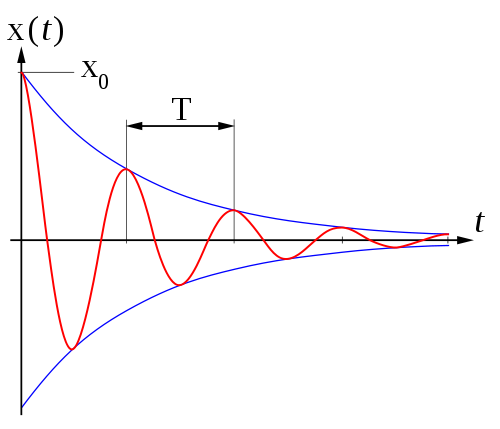
\includegraphics[scale=0.45,cfbox=black] {images/damped_harmonic_oscillator.png}}
  \caption{Damped Harmonic Oscillator Displacement Function \cite{damped_harmonic_oscillator}}
  \label{fig:critically_damped_harmonic_oscillator}
\end{figure}

\bigskip
\noindent
For the damped small-angle pendulum case the equation of motion is

\medskip
\begin{equation}
\ddot{\theta} + b \dot{\theta} + \bigg (\dfrac{g}{L} \bigg ) \theta \approx 0
\label{eqn:damped_pendulum}
\end{equation}

\medskip
\noindent
which again has the same form as Equation (\ref{eqn:damp_general_form}).

\bigskip
\noindent
Finally, a few of the analogies between mechanical
and electrical systems are shown in Table \ref{tab:analogies}.


\bigskip
\begin{table} [H]
  \centering
  \renewcommand{\arraystretch}{2.0}
     \resizebox{0.90 \textwidth}{!} {																	% resize figure if you want
     \begin{tabular} {| c | c  | c | c |}
      \hline
      {\Large \bf Mechanical Quantity}  & {\Large \bf Symbol} & {\Large \bf Electrical Quantity} & {\Large \bf Symbol}\\
      \hline \hline
      Mass & m & Inductance & L\\
      \hline
      Spring Constant & k & Capacitance & C \\
      \hline
      Force & F & Voltage & V \\
      \hline
      Velocity & v & Current & I \\
      \hline
      Damping Constant & b & Resistance & R \\
      \hline
    \end{tabular}
   }
  \caption{Analogies Between Mechanical and Electrical Harmonic Oscillators}
  \label{tab:analogies}
\end{table}


\section{Quantum Harmonic Oscillators}
\label{sec:quantum_harmonic_oscillators}
Before diving into the structure and operation
of the quantum harmonic oscillator, let's take
a minute and look at the history of how we 
got here. 


\bigskip
\noindent
We pick up this story in 1851, when Gustav Kirchhoff met Robert
Wilhelm Bunsen.  Both men had been interested in why heated
objects glowed with characteristic colors and intensities. Bunsen
had just accepted a position at the University of Heidelberg, and
Kirchhoff eventually moved to Heidelberg in 1854, beginning a
fruitful collaboration with Bunsen that resulted in the
establishment of the field of spectroscopy, which involves the
analysis of the composition of chemical compounds through the
spectra they produce \cite{wiki:kirchoff, wiki:bunsen}.

\bigskip
\noindent
Intrigued by the different colors produced when various
substances were heated in a flame, Bunsen wanted to use the
colors the colors to identify chemical elements and
compounds. Broadening the concept, Kirchhoff suggested that
Bunsen not only pay attention to the immediately visible colors
but also that he study the spectra of color components produced
by passing the light produced by each substance through a
prism. Thus was the field of spectroscopy born.

\bigskip
\noindent
In 1859, Kirchhoff noted that dark lines found in the Sun's
spectrum were further darkened when the sunlight passes through a
sodium compound heated by a bunsen burner. From this, he
concluded that the original dark lines, called Fraunhofer lines
after the scientist who discovered them, result from sodium in
the Sun's atmosphere. This opened up a new technique for
analyzing the chemical composition of stars
\cite{bunsen_and_kirchoff}.

\bigskip
\noindent
That same year Kirchhoff researched the manner in which radiation
is emitted and absorbed by various substances, and formulated
what is now known as Kirchoff's Law of Thermal Radiation
\cite{kirchoffs_law_of_thermal_radiation}: In a state of thermal
equilibrium the radiation emitted by a body is equal to the
radiation absorbed by the body. By 1860, Bunsen and Kirchhoff
were able to assign distinct spectral characteristics to a number
of metals. Together they discovered cesium (1860) and rubidium
(1861) while studying the chemical composition of the Sun via its
spectral signature.

\bigskip
\noindent
In 1862 Kirchoff introduced the concept of a "blackbody," a body
that is both a perfect emitter and absorber of heat
radiation. Later research into black body radiation was pivotal
in the the development of the quantum theories that emerged at
the beginning of the twentieth century. So how did the study of
blackbodies and blackbody radiation lead to the development of
quantum mechanics? To understand this we'll first take a closer
look at exactly what blackbodies and blackbody radiation are.

\subsection{So What Exactly are Blackbodies and Why are They Important?}
\label{subsec:black_bodies}
To start, recall that light itself is an electromagnetic wave.
In other words, light is an electric field that is oscillating.
So, if you place a charged particle in a ray of light that
particle will feel an oscillating force. The charge carried by a
particle is also the source of an electric field.  So if the
charged particle is oscillating, the electric field it generates
will also oscillate, that is, the charged particle will emit
light. Ok, but what is a blackbody?

\bigskip
\noindent
First, when light is incident on a body, three things can happen:
the body can \emph{reflect} some of all of the light, the body
can \emph{transmit} some or all of the light, or the body can
\emph{absorb} some of all of the light. A body that only absorbs
and does not reflect or transmit is called a blackbody. Any
light of any wavelength that is incident on the blackbody will
not be reflected and will not be transmitted; rather, it will
disappear inside the body.

\bigskip
\noindent
So what does it imply to say that light is absorbed by a
blackbody? Well, in both the wave and particle descriptions of
light light is a carrier of energy. So when light is absorbed by
a body, it means that the energy carried by that light is
absorbed by the body and the internal energy of the body
increases. When light interacts with the surface of the body, the
protons and electrons begin to oscillate because of the charger
they carry (sound familiar?  see Section \ref{sec:smo}); that is,
they gain kinetic energy. The bottom line is that the energy
carried by the light is transferred to kinetic energy of the
charged particles in the blackbody. Note that since the electron
is much less massive than the proton it is the electrons that
hold much of this (kinetic) energy.

\bigskip
\noindent
We know from statistical mechanics that the temperature of a body
$T$ is proportional to the average kinetic energy of the
particles in the body, that is

\begin{equation*}
T_{\text{body}} \propto \overline{\text{KE}}_{\text{particles}}
\end{equation*}

\bigskip
\noindent
So when the blackbody absorbs light, the kinetic energy of its
electrons ($\overline{\text{KE}}_{\text{particles}}$) increases
and so the temperature of the body ($T_{\text{body}}$) increases.
Since the electrons of a blackbody which have temperature will
oscillate their electric field will also oscillate and as such
they will emit light.  This light is called \emph{black body
radiation}.

\bigskip
\noindent
So blackbodies can be heated by the light that is incident on
their surfaces, but they can also be heated by other processes,
such as in stars where fusion provides the energy (somewhat
paradoxically the brightest objects (stars) are also almost
perfect blackbodies).  The effect on the electrons in the star,
however, is the same: they gain kinetic energy, they move around,
create oscillating electric fields, and light is emitted.

\bigskip
\noindent
Next we can observe that the hotter the body is the larger an
electron's kinetic energy, and therefore the larger the changes
in their electric fields.

\begin{equation*}
\begin{array}{llll}
T_{\text{body}} \uparrow  
&\Rightarrow& \overline{\text{KE}}_{\text{particles}} \uparrow
		&\qquad \mathrel{\#} \text{increase in $T_{\text{body}}$ 
		                           $\Rightarrow$ increase in average 
		                           kinetic energy ($\overline{\text{KE}}$)} \\
[5pt]	
&\Rightarrow& \overline{v}_{\text{electrons}} \uparrow
		&\qquad \mathrel{\#} \text{increase in $\overline{\text{KE}} \Rightarrow$ increase in average frequency} \\
[5pt]
&\Rightarrow& \nabla \vec{E} \uparrow
		&\qquad \mathrel{\#} \text{increase in $\overline{\text{KE}} \Rightarrow$ increase in their energy field ($\nabla \vec{E}$)} \\
[5pt]			
&\Rightarrow& P_{\text{light}} \uparrow 
		&\qquad \mathrel{\#} \text{increase in $\vec{E}$ $\Rightarrow$ increase in the power of the light emitted ($P_{\text{light}}$)} \\
[5pt]
&\Rightarrow& P_{\text{light}} = f(T)
		&\qquad \mathrel{\#} \text{the power of the light emitted from a blackbody is a function of its temperature}
\end{array}
\end{equation*}

% \bigskip
\noindent
So what we have learned is there is a direct relationship between
the temperature of the surface of the blackbody and the
intensity of the light it emits. This relationship is called
Stefan-Boltzmann's Law and is typically written as

\begin{equation}
P = \sigma A T^4
\label{eqn:stefan_boltzmanns_law}
\end{equation}

\bigskip
\noindent
In words, Equation (\ref{eqn:stefan_boltzmanns_law}) says that
the power ($P$) emitted by a blackbody is proportional to its
area ($A$) and temperature to the forth power ($T^4$).  The
proportionality constant $\sigma$ is called Stefan-Boltzmann's
constant and

\begin{equation*}
\sigma = 5.67 \times 10^{-8} W m^{-2} K^{-4}
\end{equation*}

\bigskip
\noindent
Now would be a good time to remember that a blackbody is just a
model; there is no such thing as a perfect blackbody; in reality
objects do not absorb one hundred percent of the incident
light. Rather, in real bodies there is some reflection and
transmission. Such a (real) body is called a \emph{greybody}. 
There is a quantity, emissivity, which tells us how close
a greybody is to a theoretical blackbody.

\begin{definition}
{\bf Emissivity: } An object's emissivity, $e$, measures how a
greybody's behavior compares to a theoretical blackbody.
\end{definition}

\noindent
Now we can calculate the power emitted by a greybody
as follows 

\begin{equation}
P = e\sigma A T^4
\label{eqn:grey_body_power}
\end{equation}

\medskip
\noindent
We can see that when the emissivity of an object is equal to one
($e = 1$), the object is an ideal blackbody. When the emissivity
is equal to zero ($e = 0$) we call the object is ideal white
body. Finally, if $0 < e < 1$ we call the object a greybody.

\bigskip
\noindent
Interestingly, for humans

\begin{equation*}
\begin{array}{llll}
e &=& 0.97							&\qquad \mathrel{\#} \text{humans are greybodies that are almost blackbodies} \\
[5pt]
T &=& 37^{\circ} \, C				&\qquad \mathrel{\#} \text{average human temperature is about $37^{\circ} \, C$} \\
[5pt]
P &=& e \sigma A T^4 \approx 810 W	&\qquad \mathrel{\#} \text{human emit about 810 W of electromagnetic radiation} 
\end{array}
\end{equation*}

\bigskip
\noindent
So humans do emit light, we just can't see it (it's in the
infrared part of the spectrum).  Surprisingly, animals and plants
turn out to be have high emissivity (are good blackbodies),
while minerals such as aluminium or silver have low emissivity
(high reflectivity). This is why aluminium ($e = 0.05$) is used
in household mirrors and silver ($e = 0.02$) is used in
high-grade mirrors; they are both nearly perfect reflectors.

\section{Quantum Fields}
\label{sec:quantum_fields}

\section{Conclusions}
\label{sec:conclusions}


\section*{Acknowledgements}
Thanks to Chris Lonvick (lonvick@gmail.com) for his thoughtful
suggestions on Figure \ref{fig:simple_pendulum} and to
Dave Plonka for his helpful comments on Table
\ref{tab:analogies}. Thanks also to Bill Westfield for
noticing an error in my description of the accuracy of
Huygens' pendulum clock.
%
%	LaTeX source on overleaf.com
%
\section*{\LaTeX \hspace{0.10 mm} Source}
\url{https://www.overleaf.com/read/xjmyvksvtztb}
%
%	get a bibliography
%
%	Note:.bib files go in ~/Library/texmf/bibtex/bib with TeXShop (MacTeX).
%	You can also use an absolute path, e.g. \bibliography{/Users/dmm/papers/bib/qc}
%
\bibliographystyle{plain}
\bibliography{qc}
%
%	done
%
\end{document} 

